%\todomacaluso{
%	\begin{itemize}
%		\item General description of the framework
%		\item Discussion about the motivation and the importance of this framework, such as the necessity of a Reinforcement Learning Framework to test different algorithms with different environments providing the same interface.
%		\item One contribution of the thesis: the creation and design of an OpenAI Gym environment for Anki Cozmo Environment with connection to chapter 4.
%	\end{itemize}	
%}

\chapter{Tools and Frameworks}

This chapter aims to describe the main tools and frameworks used in this thesis. The first section will describe the OpenAI Gym framework, a central toolkit for developing and comparing reinforcement learning algorithms. The second section will outline PyTorch, an optimised tensor library for deep learning using GPUs and CPUs used to build up the convolutional neural network of this work, while the explanation and description of the Anki Cozmo robot used for the autonomous self-driving experiment will occupy the last part of this chapter.

\section{OpenAI Gym}

Nowadays, OpenAI Gym \cite{openaigymgithub,openaigymdocs,openaigymwhite}, released in 2016 with its public beta, is one of the most popular toolkits and frameworks in the reinforcement learning scenario. A brief analysis of RL research and RL features could be useful to outline the motivations underlying the need for a reinforcement learning framework.

As reported previously in  \vref{ch2}, reinforcement learning is a subfield of machine learning dedicated to the world of decision making and motor control, studying how an agent can learn and improve to achieve a specific goal in a complex, usually unknown environment. RL is becoming more and more attractive for researchers because of its visionary property of being very general. An RL algorithm can be exploited to control a robot's motor in order to make it capable of running or jumping, play a videogame or board game, make critical business decisions like pricing and inventory management, but also learn how to invest in financial trading environments. The general feature of reinforcement learning became engaging thanks to the remarkable results achieved in many challenging environments, as reported in \vref{ch2}.

Despite these appealing features, the research was slowed down by other factors no less critical.
The need for better benchmarks represents the first factor. As an example, the abundant availability of conspicuous datasets like ImageNet \cite{deng2009imagenet} has driven supervised learning improvement in the research. For what concerns reinforcement learning, the nearest equivalent to supervised learning datasets would be a broad collection of different environments in order to test various algorithms with different kinds of observations or rewards.
The second withdraw of this type of approach to learning is the lack of standardisation of environments designed in publications. In reinforcement learning, subtle differences in the definition of the problem, the design of the reward function or the action space could make the difficulty of the task grow.  This fact threatens to slow down and corrupt experiments reproducibility making an objective comparison between the results of different papers almost impossible.

The need to fix both problems was the primary motivation behind the design and implementation of OpenAI Gym.

\subsection{Environments}

The agent and the environment represent the core of reinforcement learning. The choice of OpenAI was to implement and provide the abstraction mainly for environments, not for agents, leaving developers independent concerning agent interfaces, but providing a standard interface for environments. Thanks to this approach, all agents implemented with OpenAI Gym can be used with the whole set of environments provided by the framework. Therefore, it is possible to create a personalised environment to suit the needs of a specific experiment that can be used by all agents exploiting OpenAI Gym environment interfaces.

In this scenario, we realised the first contribution to our thesis. Thanks to this framework features, we implemented an OpenAI Gym environment capable of interacting with Anki Cozmo by providing a binding between the function of Cozmo SDK and the interfaces of the reinforcement learning framework. In \vref{ch4} we will provide further information and details about our contribution.

The importance related to the high quantity of environment is fundamental to build a reliable and sustainable framework for reinforcement learning algorithms. OpenAI Gym contains a various and heterogeneous environments database, ready to be used by every developed agent thanks to the standard interface offered by the framework.

\subsubsection{Interface Functions}

Exploring OpenAI Gym, it is essential to focus on the most crucial interface functions that the agent will exploit to interact with the environment.
The functions which constitute the skeleton of an OpenAI Gym environment are the following:
\begin{itemize}
	\item \texttt{def step(self, action)}: through this function, the agent can communicate the action it wants to take. The input data depends on the type and number of variables in the actions space (e.g.\ discrete or continuous). As will be discussed in \vref{ch3:observations}, the values returned by this function represent the environment state after the manipulation caused by the action of the agents. Thanks to these data, the agent will be able to select the next action following the reinforcement learning loop.
	\item \texttt{def reset(self)}: during the episode, internal variables of the environment changes, influenced by the action taken by the actor. This function allows the agent to restart the initial situation of the environment. This procedure is particularly suitable when an episode finishes and the agent has to restart the next learning episode in a brand new copy of the environment.
	\item \texttt{def render(self, mode='human', close=False)}: this function is particularly suitable for simulated environments. It enables the visual render (if available) of the environment.
	\item \texttt{def close(self)}: the final function to close the environment after all experiments and episodes.
\end{itemize}

\subsubsection{Available environments}

To date, OpenAI Gym includes the following environments:
\begin{itemize}
	\item \textbf{Algorithms}: learning to imitate computations, such as copying or reversing symbols from the input tape, is the main aim of this typology. These environments might seem easy to be solved by a computer, but it is important to remember that the objective here is to learn to solve these tasks purely from examples. Therefore, it is possible to vary the sequence length to increase or decrease task difficulties easily. 
	\item \textbf{Atari}: various videogames of Atari 2600, a home video game console developed in 1977 which spread the use of general-purpose CPUs into gaming with game code distributed through cartridges, constitute this environment section. OpenAI Gym exploits \textit{Arcade Learning Environment} (ALE) \cite{bellemare2013arcade} providing RAW pixel images or RAM as input. This database contains more than 100 different environments.
	\item \textbf{Box2D}: here is possible to find some continuous control tasks in a simple 2D simulator such as \textit{BipedalWalker}, \textit{CarRacing} and \textit{LunarLander}
	\item \textbf{Classic Control}: in this group, it is possible to find the set of problem borrowed by control theory and widely exploited in the classic reinforcement learning literature. Some task examples are balancing a pole on a cart or swing up a pendulum.
	\item \textbf{MuJoCo}: this class contains continuous control tasks running in a fast physics three-dimensional simulator called \textit{MuJoCo} which stands for \textit{Multi-Joint dynamics with Contact}. This physics engine aims to facilitate research and development in robotics, biomechanics, graphics and animation. The simulator is particularly suitable for model-based optimisation allowing to scale up computationally-intensive techniques. 
	Thanks to its features, it became useful as a source for reinforcement learning algorithms. \cite{todorov2012mujoco}
	\item \textbf{Robotics}: OpenAI released this algorithm typology to provide eight robotics environments with manipulation tasks significantly more difficult than the MoJoCo ones. It contains \textit{Fetch}, a robotic arm to move and grab objects, and \textit{ShadowHand}, a robotic hand to manipulate and grab pens, cubes and balls. \cite{ingredientsRoboticsResearch}
\end{itemize}

\subsection{Observations} \label{ch3:observations}

As reported previously, the \texttt{step(self, action)} function of the environment is the most important one because it defines the behaviour of the environment that reacts to actions of the agent. 
Indeed, the agent has to know what its actions are doing to the environment in order to stop doing random actions and start making valuable decisions.

In order to provide this type of information to the agents, the \texttt{step} function returns four relevant values that reinforcement learning algorithms can exploit to find the best action to do in the future. These values are:

\begin{itemize}
	\item \textbf{\texttt{observation (object)}}: a specific object, different for each environment which represents the observation of the environment showing the changes provoked by the action of the agent. For example, it could represent the raw pixel data from a camera, the status of a board game or physics data of a robot (joint angles and velocities).
	\item \textbf{\texttt{reward (float)}}: the value that represents the reward achieved thanks to the action taken by the agent. The reward for each action can change among environments, but this is the crucial information to enable the agent to learn.
	\item \textbf{\texttt{done (boolean)}}: this value is a simple boolean that signals the agent that the episode ended and it is time to reset the environment to start a brand new episode. 
	\item \textbf{\texttt{info (dict)}}: a Python dictionary to monitor and show diagnostic information useful for debugging. The agent could use it as additional information in the learning process, but the documentation of OpenAI Gym does not recommend to use this data in the learning process to maintain the coherence with the reinforcement learning loop. 
\end{itemize}

The last important thing to report about OpenAI Gym framework is the definition of \texttt{Spaces}. As reported in the second chapter, an environment consists of the action space and the observation space: this distinction determines the usage of a specific algorithm rather than others to solve a given task better. For this reason, OpenAI Gym provides \texttt{Discrete} and \texttt{Box} to initialise discrete and continuous spaces, respectively. It allows the user to define a lot of features useful in the learning process, such as a maximum and minimum setup or a function to sample from the defined space easily.

\section{Anki Cozmo}

Especially in the latest decades, human beings have a complicated relationship with robots: they are very fascinated by the prospect of artificial intelligence, but they are apprehensive at the same time because of the apocalyptic plot of many sci-fi films and the big promise of automation, capable of replacing human workers in the future.
However, all these concerns disappear with the palm-sized robot Cozmo, developed by the San Francisco-based company Anki and on sale since 2016.
On first sight, Cozmo might appear as one of the cutest toy robots in the market. To design this robot, Anki employed the guidance of Carlos Baena, the former Pixar animator. 
Therefore, this robot is able to interact with users using a small display screen together with audio effects to mimic human emotional reactions and responses.
The result is a toy robot WALL-E-inspired both aesthetically and personality-wise, powered up by artificial intelligence to move in the environment. Thanks to the built-in camera, Cozmo is able to remember faces and recite names, but also to plan paths and play various game with its three cubes that carry sensors and lighting.

Despite this entertaining, but not so technical facts, it hides a lot of powerful features under the hood. Anki developers produced a high-quality Python SDK to provide plenty of functions and features for Python developers. 
This section aims to outline the hardware and the software hidden underneath the cute Cozmo bodyworks, together with a comparison with the alternatives available for the reinforcement learning system designed in this thesis.

\subsection{Cozmo Architecture}

It is possible to define Cozmo as a vision-guided mobile manipulator, one of the first consumer robot which has vision among its features. However, as reported before, the features it shows during the normal toy usage, do not equal the number of interfaces and functions made available to developers. The makes Cozmo, the right robotic choice to fast prototypying computer science projects: it is the main reason why we decided to exploit Anki Cozmo instead of other alternatives.

\Vref{fig:cozmotear1,fig:cozmotear2} shows technologies, the hardware and software stack involved in the production of Cozmo.

\begin{figure}
	\tikzset{every picture/.style={line width=0.75pt}} %set default line width to 0.75pt        
	\scalebox{0.9}{
		\centering
		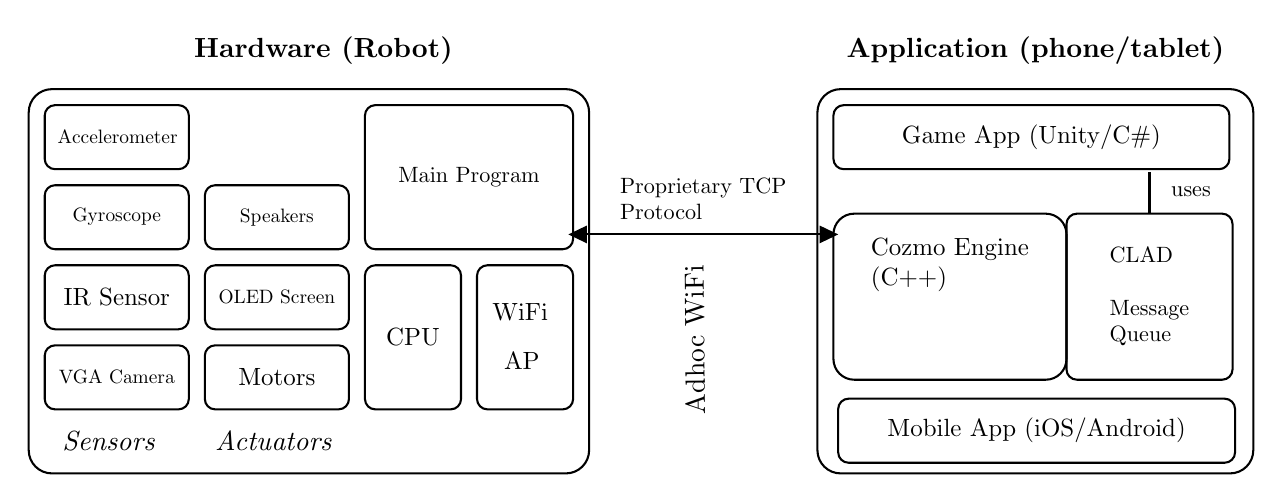
\begin{tikzpicture}[x=0.75pt,y=0.75pt,yscale=-1,xscale=1]
			%uncomment if require: \path (0,466); %set diagram left start at 0, and has height of 466
			
			%Shape: Rectangle [id:dp32857133822425977] 
			\draw  [fill={rgb, 255:red, 255; green, 255; blue, 255 }  ,fill opacity=1 ] (17.71,52.71) .. controls (17.71,49.95) and (19.95,47.71) .. (22.71,47.71) -- (82.14,47.71) .. controls (84.9,47.71) and (87.14,49.95) .. (87.14,52.71) -- (87.14,73.57) .. controls (87.14,76.33) and (84.9,78.57) .. (82.14,78.57) -- (22.71,78.57) .. controls (19.95,78.57) and (17.71,76.33) .. (17.71,73.57) -- cycle ;
			%Shape: Rectangle [id:dp46039429837534274] 
			\draw   (17.71,91.29) .. controls (17.71,88.52) and (19.95,86.29) .. (22.71,86.29) -- (82.14,86.29) .. controls (84.9,86.29) and (87.14,88.52) .. (87.14,91.29) -- (87.14,112.14) .. controls (87.14,114.9) and (84.9,117.14) .. (82.14,117.14) -- (22.71,117.14) .. controls (19.95,117.14) and (17.71,114.9) .. (17.71,112.14) -- cycle ;
			%Shape: Rectangle [id:dp38741871235010394] 
			\draw   (17.71,129.86) .. controls (17.71,127.1) and (19.95,124.86) .. (22.71,124.86) -- (82.14,124.86) .. controls (84.9,124.86) and (87.14,127.1) .. (87.14,129.86) -- (87.14,150.71) .. controls (87.14,153.48) and (84.9,155.71) .. (82.14,155.71) -- (22.71,155.71) .. controls (19.95,155.71) and (17.71,153.48) .. (17.71,150.71) -- cycle ;
			%Shape: Rectangle [id:dp004700439400786571] 
			\draw   (17.71,168.43) .. controls (17.71,165.67) and (19.95,163.43) .. (22.71,163.43) -- (82.14,163.43) .. controls (84.9,163.43) and (87.14,165.67) .. (87.14,168.43) -- (87.14,189.29) .. controls (87.14,192.05) and (84.9,194.29) .. (82.14,194.29) -- (22.71,194.29) .. controls (19.95,194.29) and (17.71,192.05) .. (17.71,189.29) -- cycle ;
			%Shape: Rectangle [id:dp6758338534339963] 
			\draw   (94.86,91.29) .. controls (94.86,88.52) and (97.1,86.29) .. (99.86,86.29) -- (159.29,86.29) .. controls (162.05,86.29) and (164.29,88.52) .. (164.29,91.29) -- (164.29,112.14) .. controls (164.29,114.9) and (162.05,117.14) .. (159.29,117.14) -- (99.86,117.14) .. controls (97.1,117.14) and (94.86,114.9) .. (94.86,112.14) -- cycle ;
			%Shape: Rectangle [id:dp39145715867558895] 
			\draw   (94.86,129.86) .. controls (94.86,127.1) and (97.1,124.86) .. (99.86,124.86) -- (159.29,124.86) .. controls (162.05,124.86) and (164.29,127.1) .. (164.29,129.86) -- (164.29,150.71) .. controls (164.29,153.48) and (162.05,155.71) .. (159.29,155.71) -- (99.86,155.71) .. controls (97.1,155.71) and (94.86,153.48) .. (94.86,150.71) -- cycle ;
			%Shape: Rectangle [id:dp4252881368662953] 
			\draw   (94.86,168.43) .. controls (94.86,165.67) and (97.1,163.43) .. (99.86,163.43) -- (159.29,163.43) .. controls (162.05,163.43) and (164.29,165.67) .. (164.29,168.43) -- (164.29,189.29) .. controls (164.29,192.05) and (162.05,194.29) .. (159.29,194.29) -- (99.86,194.29) .. controls (97.1,194.29) and (94.86,192.05) .. (94.86,189.29) -- cycle ;
			%Shape: Rectangle [id:dp8211794883898887] 
			\draw   (172,129.86) .. controls (172,127.1) and (174.24,124.86) .. (177,124.86) -- (213.29,124.86) .. controls (216.05,124.86) and (218.29,127.1) .. (218.29,129.86) -- (218.29,189.29) .. controls (218.29,192.05) and (216.05,194.29) .. (213.29,194.29) -- (177,194.29) .. controls (174.24,194.29) and (172,192.05) .. (172,189.29) -- cycle ;
			%Shape: Rectangle [id:dp01326013235082557] 
			\draw   (226,129.86) .. controls (226,127.1) and (228.24,124.86) .. (231,124.86) -- (267.29,124.86) .. controls (270.05,124.86) and (272.29,127.1) .. (272.29,129.86) -- (272.29,189.29) .. controls (272.29,192.05) and (270.05,194.29) .. (267.29,194.29) -- (231,194.29) .. controls (228.24,194.29) and (226,192.05) .. (226,189.29) -- cycle ;
			%Shape: Rectangle [id:dp7658070686999401] 
			\draw   (172,52.71) .. controls (172,49.95) and (174.24,47.71) .. (177,47.71) -- (267.29,47.71) .. controls (270.05,47.71) and (272.29,49.95) .. (272.29,52.71) -- (272.29,112.14) .. controls (272.29,114.9) and (270.05,117.14) .. (267.29,117.14) -- (177,117.14) .. controls (174.24,117.14) and (172,114.9) .. (172,112.14) -- cycle ;
			%Rounded Rect [id:dp6707545818557623] 
			\draw   (10,51.19) .. controls (10,45.01) and (15.01,40) .. (21.19,40) -- (268.81,40) .. controls (274.99,40) and (280,45.01) .. (280,51.19) -- (280,213.96) .. controls (280,220.13) and (274.99,225.14) .. (268.81,225.14) -- (21.19,225.14) .. controls (15.01,225.14) and (10,220.13) .. (10,213.96) -- cycle ;
			%Shape: Rectangle [id:dp1247876053058975] 
			\draw   (397.71,52.71) .. controls (397.71,49.95) and (399.95,47.71) .. (402.71,47.71) -- (583.5,47.71) .. controls (586.26,47.71) and (588.5,49.95) .. (588.5,52.71) -- (588.5,73.57) .. controls (588.5,76.33) and (586.26,78.57) .. (583.5,78.57) -- (402.71,78.57) .. controls (399.95,78.57) and (397.71,76.33) .. (397.71,73.57) -- cycle ;
			%Shape: Rectangle [id:dp5285084620933563] 
			\draw   (397.71,110) .. controls (397.71,104.48) and (402.19,100) .. (407.71,100) -- (500,100) .. controls (505.52,100) and (510,104.48) .. (510,110) -- (510,170) .. controls (510,175.52) and (505.52,180) .. (500,180) -- (407.71,180) .. controls (402.19,180) and (397.71,175.52) .. (397.71,170) -- cycle ;
			%Shape: Rectangle [id:dp1411259106243823] 
			\draw   (400,194.14) .. controls (400,191.38) and (402.24,189.14) .. (405,189.14) -- (586.21,189.14) .. controls (588.97,189.14) and (591.21,191.38) .. (591.21,194.14) -- (591.21,215) .. controls (591.21,217.76) and (588.97,220) .. (586.21,220) -- (405,220) .. controls (402.24,220) and (400,217.76) .. (400,215) -- cycle ;
			%Rounded Rect [id:dp924085976000878] 
			\draw   (390,51.19) .. controls (390,45.01) and (395.01,40) .. (401.19,40) -- (588.81,40) .. controls (594.99,40) and (600,45.01) .. (600,51.19) -- (600,213.96) .. controls (600,220.13) and (594.99,225.14) .. (588.81,225.14) -- (401.19,225.14) .. controls (395.01,225.14) and (390,220.13) .. (390,213.96) -- cycle ;
			%Shape: Rectangle [id:dp5178962107538444] 
			\draw   (510,105) .. controls (510,102.24) and (512.24,100) .. (515,100) -- (585,100) .. controls (587.76,100) and (590,102.24) .. (590,105) -- (590,175) .. controls (590,177.76) and (587.76,180) .. (585,180) -- (515,180) .. controls (512.24,180) and (510,177.76) .. (510,175) -- cycle ;
			%Straight Lines [id:da3605271488149666] 
			\draw    (550,80) -- (550,100) ;
			
			
			%Straight Lines [id:da2112054558095744] 
			\draw    (273,110) -- (397,110) ;
			\draw [shift={(400,110)}, rotate = 180] [fill={rgb, 255:red, 0; green, 0; blue, 0 }  ][line width=0.08]  [draw opacity=0] (8.93,-4.29) -- (0,0) -- (8.93,4.29) -- cycle    ;
			\draw [shift={(270,110)}, rotate = 0] [fill={rgb, 255:red, 0; green, 0; blue, 0 }  ][line width=0.08]  [draw opacity=0] (8.93,-4.29) -- (0,0) -- (8.93,4.29) -- cycle    ;
			
			% Text Node
			\draw (52.81,62.76) node  [scale=0.7] [align=left] {Accelerometer};
			% Text Node
			\draw (52.43,101.71) node  [scale=0.7] [align=left] {Gyroscope};
			% Text Node
			\draw (52.43,140.29) node  [scale=0.9] [align=left] {IR Sensor};
			% Text Node
			\draw (52.43,178.86) node  [scale=0.7] [align=left] {VGA Camera};
			% Text Node
			\draw (129.57,101.71) node  [scale=0.7] [align=left] {Speakers};
			% Text Node
			\draw (129.57,140.29) node  [scale=0.7] [align=left] {OLED Screen};
			% Text Node
			\draw (129.57,178.86) node  [scale=0.9] [align=left] {Motors};
			% Text Node
			\draw (195.14,159.57) node  [scale=0.9] [align=left] {CPU};
			% Text Node
			\draw (246.83,147.61) node  [scale=0.9] [align=left] {WiFi};
			% Text Node
			\draw (247.6,170.76) node  [scale=0.9] [align=left] {AP};
			% Text Node
			\draw (222.14,82.43) node  [scale=0.8] [align=left] {Main Program};
			% Text Node
			\draw (48.96,209.33) node   [align=left] {\textit{Sensors}};
			% Text Node
			\draw (128.41,209.33) node   [align=left] {\textit{Actuators}};
			% Text Node
			\draw (493.11,63.14) node  [scale=0.9] [align=left] {Game App (Unity/C\#)};
			% Text Node
			\draw (453.86,124.71) node  [scale=0.9] [align=left] {Cozmo Engine\\(C++)};
			% Text Node
			\draw (495.61,204.57) node  [scale=0.9] [align=left] {Mobile App (iOS/Android)};
			% Text Node
			\draw (550,140) node  [scale=0.8] [align=left] {CLAD\\\\Message\\Queue};
			% Text Node
			\draw (570,89.5) node  [scale=0.8] [align=left] {uses};
			% Text Node
			\draw (335,93) node  [scale=0.8] [align=left] {Proprietary TCP\\Protocol};
			% Text Node
			\draw (330.9,160.6) node  [rotate=-269.43] [align=left] {Adhoc WiFi};
			% Text Node
			\draw (152,21.5) node   [align=left] {\textbf{Hardware (Robot)}};
			% Text Node
			\draw (495,21.5) node   [align=left] {\textbf{Application (phone/tablet)}};
			
			\end{tikzpicture}
			}
		\caption[Interaction Robot/Application]{Interaction between the Robot and the mobile application stack. \cite{mellon2017cognitive}}
		\label{fig:cozmotear1}
	\end{figure}

	Starting from \vref{fig:cozmotear1}, it is noticeable that Cozmo has a lot of sensors and actuators, which enable it to move and understand the surrounding environment. For what concerns the sensor part, the VGA Camera is the crucial component exploited in the thesis. This camera provides a grayscale image with 320$\times$240. Anki reported a camera resolution equal to 640$\times$480, but the firmware supports only the lower resolution. Furthermore, the camera can detect and acquire colours, but the firmware limits this feature to maintain the bandwidth stable and avoid overloads or slowdowns in the communication with the mobile application and subsequently, the user program running on the computer. 
	The camera has approximately 60° field of view (FOV) and 290mm focal length.
	
	As regards actuators column, Cozmo can explore the world thanks to with four motors and over fifty gears. It has no wheels, but two tracks: Cozmo can steer and move freely by managing the speed of the individual tracks.
	Another moving part is the head that can move up or down to direct the camera and the display. It also has a forklift with which it can lift objects or cubes available.





\begin{figure}
	\tikzset{every picture/.style={line width=0.75pt}} %set default line width to 0.75pt        
\scalebox{0.9}{
\centering		
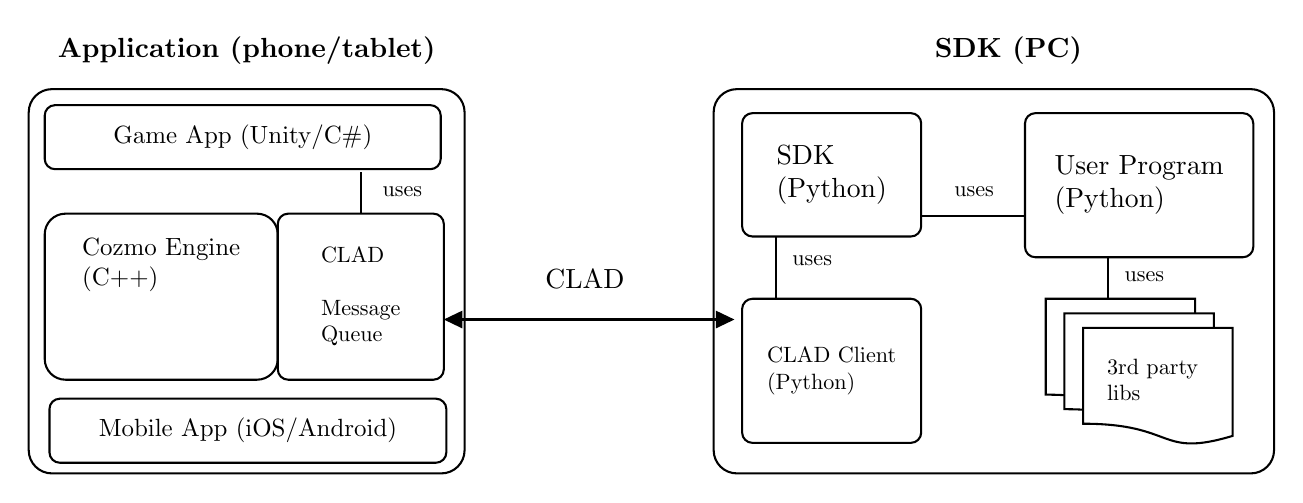
\begin{tikzpicture}[x=0.75pt,y=0.75pt,yscale=-1,xscale=1]
	%uncomment if require: \path (0,466); %set diagram left start at 0, and has height of 466
	
	%Shape: Rectangle [id:dp01326013235082557] 
	\draw   (353.71,55.57) .. controls (353.71,52.81) and (355.95,50.57) .. (358.71,50.57) -- (435,50.57) .. controls (437.76,50.57) and (440,52.81) .. (440,55.57) -- (440,105) .. controls (440,107.76) and (437.76,110) .. (435,110) -- (358.71,110) .. controls (355.95,110) and (353.71,107.76) .. (353.71,105) -- cycle ;
	%Rounded Rect [id:dp6707545818557623] 
	\draw   (340,50.19) .. controls (340,44.01) and (345.01,39) .. (351.19,39) -- (598.81,39) .. controls (604.99,39) and (610,44.01) .. (610,50.19) -- (610,212.96) .. controls (610,219.13) and (604.99,224.14) .. (598.81,224.14) -- (351.19,224.14) .. controls (345.01,224.14) and (340,219.13) .. (340,212.96) -- cycle ;
	%Shape: Rectangle [id:dp1247876053058975] 
	\draw   (17.71,51.71) .. controls (17.71,48.95) and (19.95,46.71) .. (22.71,46.71) -- (203.5,46.71) .. controls (206.26,46.71) and (208.5,48.95) .. (208.5,51.71) -- (208.5,72.57) .. controls (208.5,75.33) and (206.26,77.57) .. (203.5,77.57) -- (22.71,77.57) .. controls (19.95,77.57) and (17.71,75.33) .. (17.71,72.57) -- cycle ;
	%Shape: Rectangle [id:dp5285084620933563] 
	\draw   (17.71,109) .. controls (17.71,103.48) and (22.19,99) .. (27.71,99) -- (120,99) .. controls (125.52,99) and (130,103.48) .. (130,109) -- (130,169) .. controls (130,174.52) and (125.52,179) .. (120,179) -- (27.71,179) .. controls (22.19,179) and (17.71,174.52) .. (17.71,169) -- cycle ;
	%Shape: Rectangle [id:dp1411259106243823] 
	\draw   (20,193.14) .. controls (20,190.38) and (22.24,188.14) .. (25,188.14) -- (206.21,188.14) .. controls (208.97,188.14) and (211.21,190.38) .. (211.21,193.14) -- (211.21,214) .. controls (211.21,216.76) and (208.97,219) .. (206.21,219) -- (25,219) .. controls (22.24,219) and (20,216.76) .. (20,214) -- cycle ;
	%Rounded Rect [id:dp924085976000878] 
	\draw   (10,50.19) .. controls (10,44.01) and (15.01,39) .. (21.19,39) -- (208.81,39) .. controls (214.99,39) and (220,44.01) .. (220,50.19) -- (220,212.96) .. controls (220,219.13) and (214.99,224.14) .. (208.81,224.14) -- (21.19,224.14) .. controls (15.01,224.14) and (10,219.13) .. (10,212.96) -- cycle ;
	%Shape: Rectangle [id:dp5178962107538444] 
	\draw   (130,104) .. controls (130,101.24) and (132.24,99) .. (135,99) -- (205,99) .. controls (207.76,99) and (210,101.24) .. (210,104) -- (210,174) .. controls (210,176.76) and (207.76,179) .. (205,179) -- (135,179) .. controls (132.24,179) and (130,176.76) .. (130,174) -- cycle ;
	%Straight Lines [id:da3605271488149666] 
	\draw    (170,79) -- (170,99) ;
	
	
	%Shape: Rectangle [id:dp18789236199658887] 
	\draw   (490,55.57) .. controls (490,52.81) and (492.24,50.57) .. (495,50.57) -- (595,50.57) .. controls (597.76,50.57) and (600,52.81) .. (600,55.57) -- (600,115) .. controls (600,117.76) and (597.76,120) .. (595,120) -- (495,120) .. controls (492.24,120) and (490,117.76) .. (490,115) -- cycle ;
	%Shape: Rectangle [id:dp06226066777668593] 
	\draw   (353.71,145) .. controls (353.71,142.24) and (355.95,140) .. (358.71,140) -- (435,140) .. controls (437.76,140) and (440,142.24) .. (440,145) -- (440,204.43) .. controls (440,207.19) and (437.76,209.43) .. (435,209.43) -- (358.71,209.43) .. controls (355.95,209.43) and (353.71,207.19) .. (353.71,204.43) -- cycle ;
	%Straight Lines [id:da26247537190243575] 
	\draw    (213,150) -- (347,150) ;
	\draw [shift={(350,150)}, rotate = 180] [fill={rgb, 255:red, 0; green, 0; blue, 0 }  ][line width=0.08]  [draw opacity=0] (8.93,-4.29) -- (0,0) -- (8.93,4.29) -- cycle    ;
	\draw [shift={(210,150)}, rotate = 0] [fill={rgb, 255:red, 0; green, 0; blue, 0 }  ][line width=0.08]  [draw opacity=0] (8.93,-4.29) -- (0,0) -- (8.93,4.29) -- cycle    ;
	%Straight Lines [id:da8910764864061073] 
	\draw    (370,110) -- (370,140) ;
	
	
	%Straight Lines [id:da7025332895008514] 
	\draw    (490,100) -- (440,100) ;
	
	
	%Flowchart: Multidocument [id:dp4320351285174221] 
	\draw  [fill={rgb, 255:red, 255; green, 255; blue, 255 }  ,fill opacity=1 ] (572,140) -- (500,140) -- (500,186.2) .. controls (545,186.2) and (536,202.86) .. (572,192.08) -- cycle ; \draw  [fill={rgb, 255:red, 255; green, 255; blue, 255 }  ,fill opacity=1 ] (581,147) -- (509,147) -- (509,193.2) .. controls (554,193.2) and (545,209.86) .. (581,199.08) -- cycle ; \draw  [fill={rgb, 255:red, 255; green, 255; blue, 255 }  ,fill opacity=1 ] (590,154) -- (518,154) -- (518,200.2) .. controls (563,200.2) and (554,216.86) .. (590,206.08) -- cycle ;
	%Straight Lines [id:da0995629449951837] 
	\draw    (530,120) -- (530,140) ;
	
	
	
	% Text Node
	\draw (113.11,62.14) node  [scale=0.9] [align=left] {Game App (Unity/C\#)};
	% Text Node
	\draw (73.86,123.71) node  [scale=0.9] [align=left] {Cozmo Engine\\(C++)};
	% Text Node
	\draw (115.61,203.57) node  [scale=0.9] [align=left] {Mobile App (iOS/Android)};
	% Text Node
	\draw (170,139) node  [scale=0.8] [align=left] {CLAD\\\\Message\\Queue};
	% Text Node
	\draw (190,88.5) node  [scale=0.8] [align=left] {uses};
	% Text Node
	\draw (482,20.5) node   [align=left] {\textbf{SDK (PC)}};
	% Text Node
	\draw (115,20.5) node   [align=left] {\textbf{Application (phone/tablet)}};
	% Text Node
	\draw (396.86,80.29) node   [align=left] {SDK\\(Python)};
	% Text Node
	\draw (545,85.29) node   [align=left] {User Program\\(Python)};
	% Text Node
	\draw (396.86,174.71) node  [scale=0.8] [align=left] {CLAD Client\\(Python)};
	% Text Node
	\draw (387.5,121.5) node  [scale=0.8] [align=left] {uses};
	% Text Node
	\draw (465.5,88.5) node  [scale=0.8] [align=left] {uses};
	% Text Node
	\draw (551.5,179) node   [scale=0.8,align=left] {3rd party\\libs};
	% Text Node
	\draw (547.5,129.5) node  [scale=0.8] [align=left] {uses};
	% Text Node
	\draw (278,130.5) node   [align=left] {CLAD};
	\end{tikzpicture}
	}
	\caption[Interaction Application/PC]{Interaction between the mobile application stack and the Python user program. \cite{mellon2017cognitive}}
	\label{fig:cozmotear2}
\end{figure}

\subsection{Why Cozmo?}


\section{PyTorch}


\todomacaluso{
	\begin{itemize}
		\item General description of Pytorch framework
	\end{itemize}	
}



\subsection{Tensor and Gradients}



\subsection{Building a Convolutional Neural Network}



\subsection{Loss function and Optimizers}



\subsection{TensorboardX}


